% Should be <2 pages
\iffalse
\begin{itemize}
	\item How to measure simplicity and scalability
	\item Not just what you did but why and what the consequences are
\end{itemize}
Explore design space, motivate method, consequences, 
\fi

\section{Data Reading Interval}
\subsection{Behaviors}

\begin{figure}[H]
\centering
	\begin{subfigure}[b]{0.3\textwidth}
    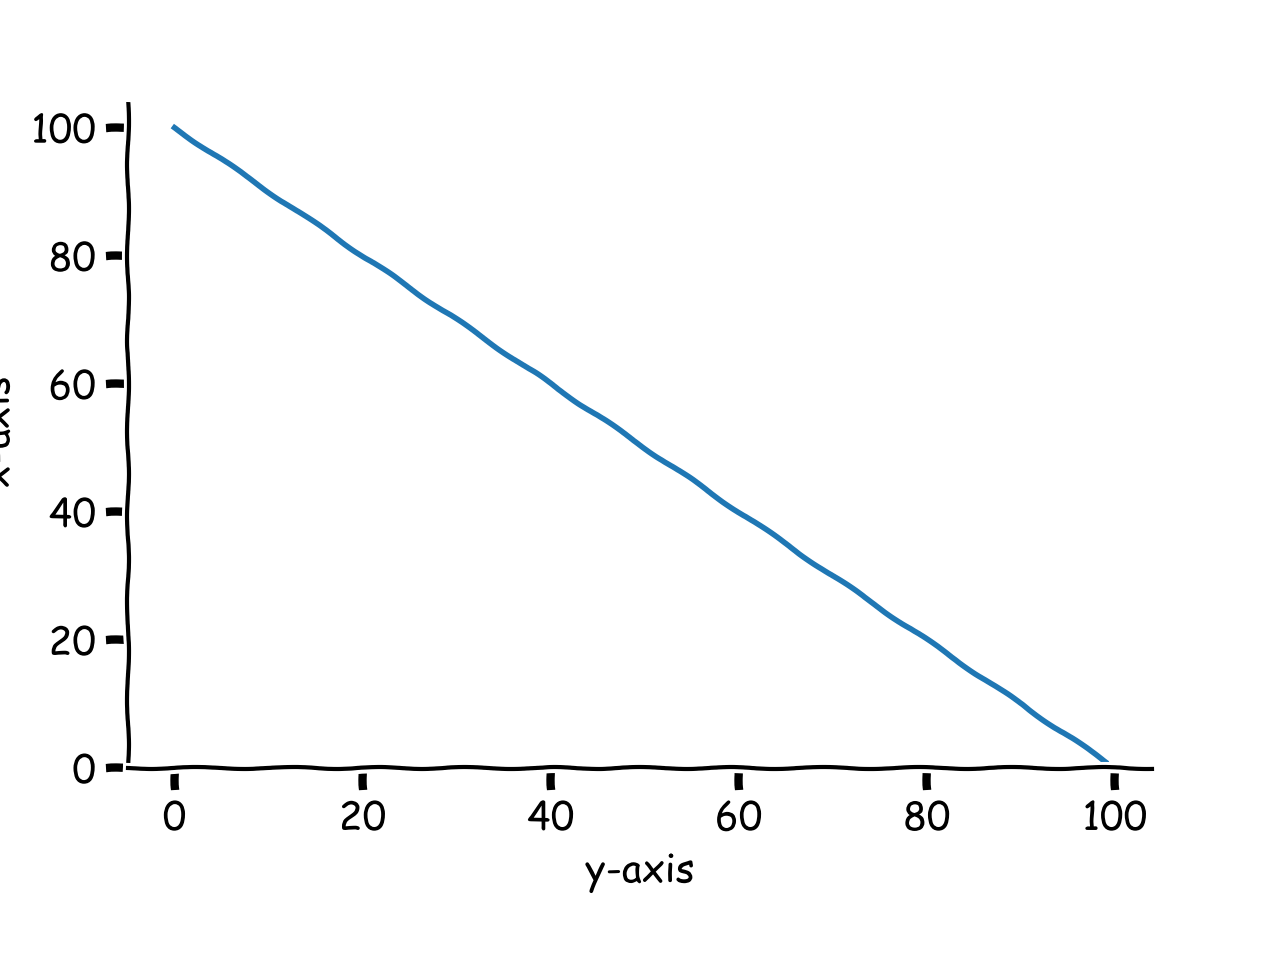
\includegraphics[width=\textwidth]{linear.png}
    \caption{Graph with linear decrease}
    \label{fig:linear}
	\end{subfigure}
	%
	\begin{subfigure}[b]{0.3\textwidth}
    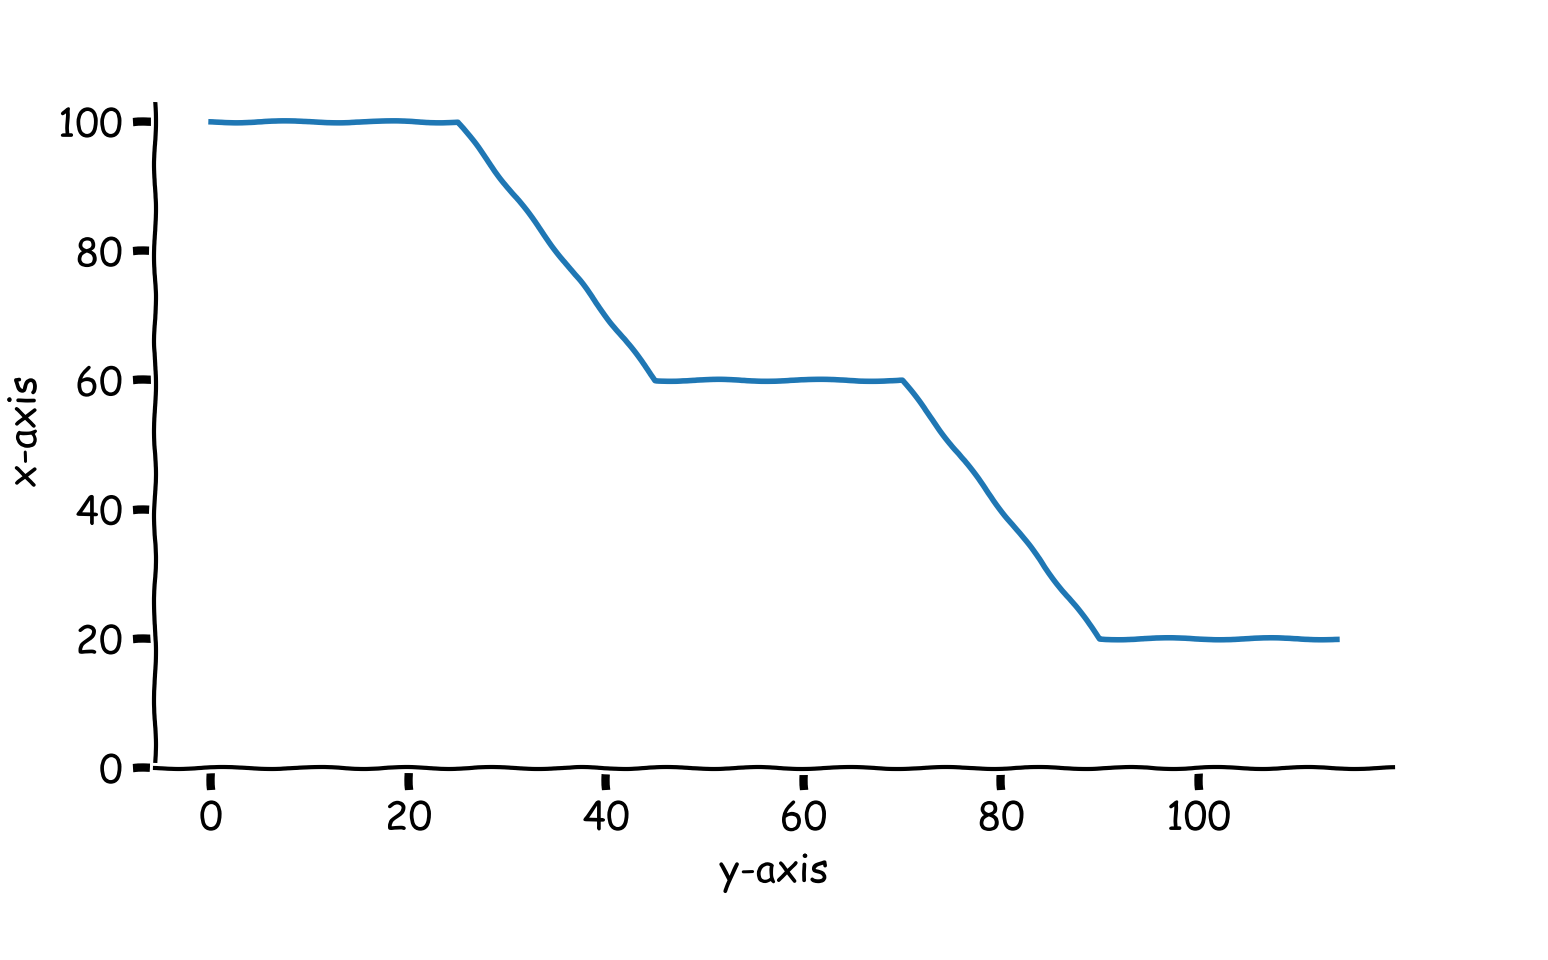
\includegraphics[width=\textwidth]{plateu.png}
    \caption{Graph with plateaus}
    \label{fig:plat}
	\end{subfigure}
	%
	\begin{subfigure}[b]{0.3\textwidth}
    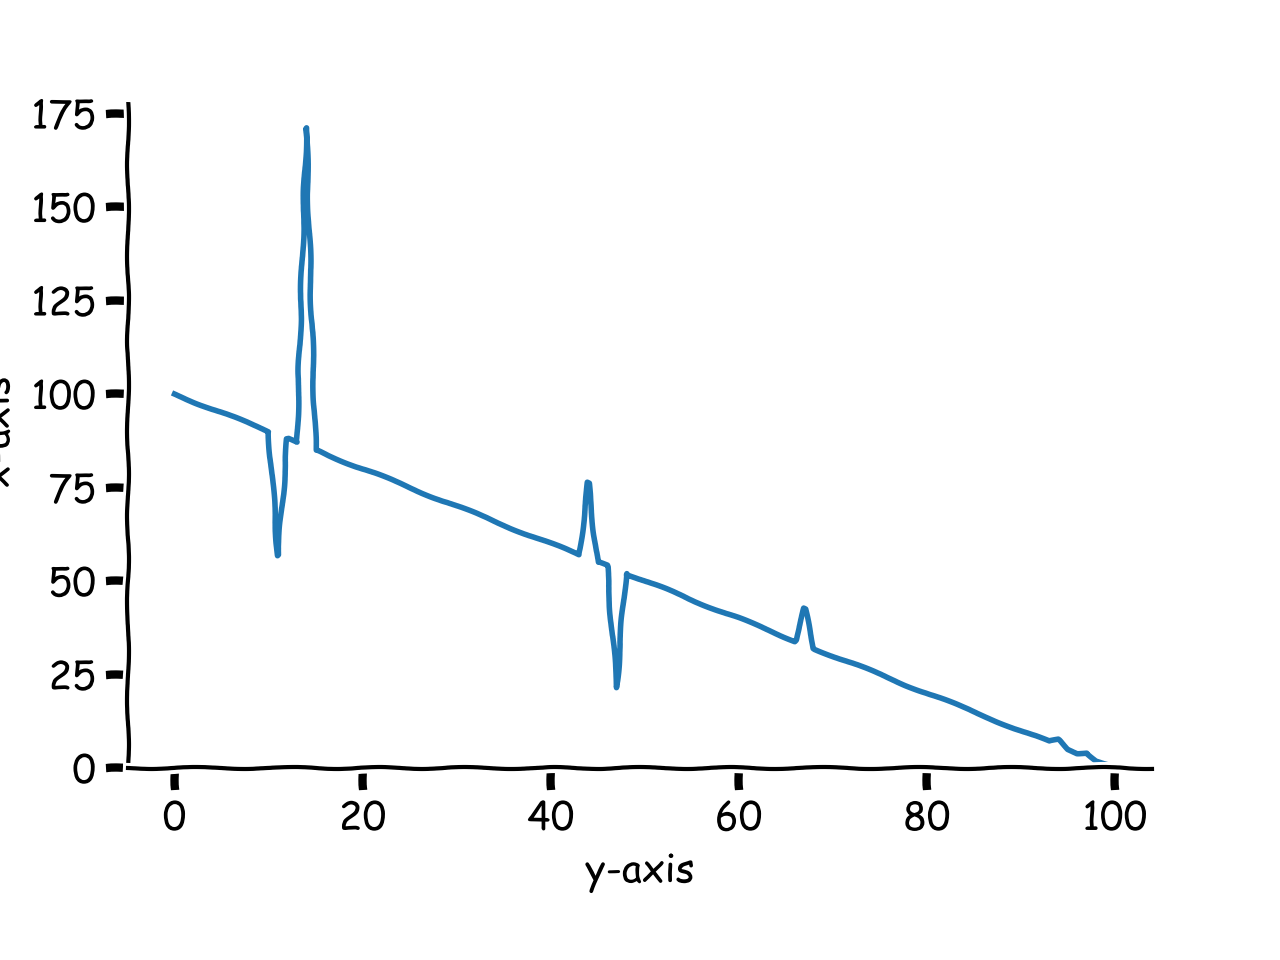
\includegraphics[width=\textwidth]{spikes.png}
    \caption{Graph with spikes}
    \label{fig:spikes}
	\end{subfigure}
\end{figure}

To determine what we want to achieve in this aspect, it's useful to first define some behaviors from which we will base our assumptions on. In figure \ref{fig:linear} we see our base case, with a simple linear decline in data values. In figure \ref{fig:plat} we see data the goes through some changes periodically, but stabilizes itself between the changes. In figure \ref{fig:spikes} we see a clear linear decrease with some spikes in data values here and there, which we can assume to be faulty measurements.

\subsection{Implementation}
We're interested in modifying the data reading rate depending on the changes in data values. This can be done in a number of ways, but a simple start might be to measure the delta in the last \textit{x} amount of values and increase/decrease the interval depending on it's relation to delta. 

To do this we need a \textit{short term buffer} of a fixed size that contains \textit{x} amount of recently read values in chronological order. This buffer should act as a FIFO-queue, so that the first element added to the buffer is the first one removed during an overflow. Measuring the delta of all the values in the buffer, we compare it to a threshold value that will either decrease, increase or maintain the current interval of reading data. When we say the delta of \textit{all} values in the buffer, we mean the delta between each data point summed up. Assuming a buffer of 10 values, we would calculate the sum as follows:

$$\sum_{n=0}^{8} x_n - x_{n+1}$$

Starting with figure \ref{fig:linear}, the values go from (100-0) in 100 data points on the x-axis. Calculating the delta for the first 10 values would be simple. The short term buffer would be: [100, 99, ..., 91]. The total delta would be (100-99) + (99 - 98) + ... + (92 - 91) = 10. For this example we can say that our determined threshold for decreasing our reading interval is $\geq 15$, and an increase at $\leq 5$. In our current example the reading interval is maintained. 

In figure \ref{fig:plat} the slopes are steeper, and would thus generate a larger total delta. Assuming a buffer length of 10, the first 5 values would be 100, and the other 5 would be 75. Our delta calculation would give us a value of 25, which would 



\section{Sensor Failure}

\section{Sensor Disconnect}